 \chapter{Flow Monitoring Performance}\label{chap:flow-monitoring-performance}

\begin{chapintro}

Intro, flow monitoring on commodity hardware, possibly using HW accelerated NIC.

The paper included in this chapter is~\cite{Velan-2015-High}. Another paper related to this chapter is~\cite{Pus-2015-Hardware}.

The organisation of this chapter is as follows:
\begin{itemize}
  \item Section~\ref{sec:performance-measurement} provides background to the measurement of flow monitoring performance and highlight its pitfalls.
  \item Section~\ref{sec:performance-capture} describes the state of the art of high-speed packet capture, which is an important part of every flow monitoring system.
  \item Section~\ref{sec:performance-hw-acceleration} shows how can the flow monitoring be accelerated with the use of specialized FPGA-based network interface cards.
  \item Section~\ref{sec:performance-sw-optimization} discusses available methods of optimization of flow exporter software.
  \item Section~\ref{sec:performance-high-density} presents a high-density flow monitoring system capable of monitoring of sixteen 10\,Gb links in a single box and evaluates its performance.
  \item Section~\ref{sec:performance-summary} summarizes the chapter.
\end{itemize}

\end{chapintro}

\newpage


\section{Measuring Flow Monitoring Performance}\label{sec:performance-measurement}

The primary goal of measuring flow monitoring performance is to determine whether the system can be deployed to monitor a particular network or a link. For example, if the system is capable of monitoring 20\,Gb/s of traffic, it can be deployed on both directions of a 10\,Gb/s link. However, the claim that the system can handle 20\,Gb/s may mean a lot of different things and it usually differs from vendor to vendor. The throughput of a flow monitoring process depends on a number of factors, such as configuration of the flow creation process and type of network traffic that is being monitored. 10\,Gb/s may mean 14.88\,Mpps (millions of packets per second) for minimum Ethernet frames (20\,B + 64\,B) or just 813\,kpps for maximum Ethernet frames on 1500\,MTU (each frame is 1538\,B). The processing of different packet headers can take different time as well, for example IPv4 vs IPv6 or UDP vs TCP. The number of flows has a large impact on the flow creation process as a flow record must be kept for each of the flows. Therefore, a detailed performance analysis of the flow monitoring system should be performed before its real-world deployment.

The throughput of the flow monitoring system is usually measured either in packets per second or bits per second. However, since the packet size should be reported as well so that these values provide meaningful information, they are mostly interchangeable. Packets per second metric is preferred in most of this chapter.

The goal of this section is two-fold. Firstly, it describes the parameters that need to be specified when reporting on a flow monitoring system performance. There are three different categories of the parameters: hardware configuration, exporter configuration, traffic composition. Secondly, measurement of impact of optimizations is discussed. Although the impact can be measured simply by an increase in the overall throughput, there are a few pitfalls that need to be recognized and avoided for the results to be interpreted correctly.


\subsection{Measuring Overall Throughput}

The overall throughput of the flow monitoring process depends upon a number of factors. Moreover there are two methods of measuring the throughput even if all of these factors are set. The first method is to generate the testing traffic in such a rate that is above the capability of the monitoring process to handle. The throughput is then determined as the number of packets that were actually processed by the flow exporter. This method gives an upper bound on the capabilities of the monitoring process and the measurement is quite easy to carry out. However, deploying the flow monitoring system based on such an estimate can easily lead to dropped packets in practice since there is quite a large packet drop associated with the measurement as well. The second method measures throughput without packet loss or with a defined packet loss rate. Given a predetermined packet loss rate, the traffic is generated so that the flow monitoring system performs with lower that given packet loss rate. The throughput is then increased until the packet loss matches the predetermined value and the throughput at that point is considered to be the result of the measurement. Both performance measurement methods are important. The first one gives an upper bound of the capabilities of the flow monitoring process and the second one shows how much traffic can be safely processed with acceptable packet loss.

When evaluating the performance of a flow monitoring process, the hardware on which it runs must be taken into consideration. The performance depends on the frequency of the processor, available instruction sets and size of caches. When the exporter software is able to utilize multiple threads the number of cores of the processor and the number of processors matter as well. Moreover, when there are more than one processor, the correct use of Non-Uniform Memory Access (NUMA) architecture is important. The buffers of processes and threads running on a one CPU should be in a memory connected to the same CPU. Otherwise the latency for accessing this memory is increased as the data must be accessed by a memory controller of another process through a bus such, as the QuickPath Interconnect~\cite{IntelCorporation-2009-Introduction} bus or its newer version Ultra Path Interconnect (in case of Intel processors).

The choice of packet capture solution often limits the upper bound on the throughput of the flow monitoring process. Although packet capture is an important part of flow monitoring process, it is used for other tasks as well and is of interest to various researchers~\cite{Garcia-Dorado-2013-High, Nassopulos-2014-Flow}. High-speed packet capture is described in more detail in Section~\ref{sec:performance-capture}.

The configuration of the flow exporter has a great impact on the throughput as well. The active and inactive timeouts significantly affect the number of created flows and flow records~\cite{Hofstede-2014-Flow} which in turn affects the utilization of the flow cache and therefore the total throughput. The flow cache size should be tuned to the expected number of flows so that the data locality is preserved as much as possible. Moreover, the size of flow records depends on the number of extracted properties and it affects the size of the cache as well. The more properties extracted, the larger the flow record. Naturally, the number of extracted properties has a direct impact on the throughput since each property must be extracted and stored in the flow record, which requires computing power and more memory accesses.

One of the most important aspects of throughput measurement is the used dataset. Choosing shortest packets and a single flow allows to benchmark the packet parser, shortest packets and a large number of flows put great stress on the flow cache. Using more complex packets with multiple protocol layers tests the packet parser capabilities and performance as well. The relative sizes of flows in the data set matter as well. When there are a few dominant flows, the corresponding flow records are kept cached and the overall performance increases. However, if the packets of the flows are equally interlaced, the caching of the flow records is limited. Since the choice of the dataset has such an extensive impact on the flow monitoring process and its throughput, it is imperative to choose a correct dataset that supports the intentions of the given benchmark. A guidance for choosing a dataset can be found in the work of the IETF Internet IP Performance Measurement working group~\cite{IESG-1997-IP} and IETF Benchmarking Methodology working group~\cite{IESG-1989-Benchmarking}, especially in~\cite{rfc2330, rfc6985}.

We have argued that there are many factors that influence the throughput of a flow monitoring system. Since it is clearly not possible to test all combinations of the input parameters, it is necessary to choose a set of appropriate settings that cover either the most extreme scenarios or approximate some important real world scenario. The work of~\citeauthor{Nassopulos-2014-Flow}~\cite{Nassopulos-2014-Flow} shows that performing a measurement using a large number of configurations allows to derive results that can help with the optimization effort. They show that the implementation of the flow cache as well as the composition of the traffic has large impact on the flow monitoring process. Regardless of the chosen parameters, a proper description of the used configuration and dataset must always accompany all presented results. Therefore, we recommend to use a synthetic dataset that can be described in a few simple rules.


\subsection{Measuring an Impact of Optimizations}

Throughput measurement is an integral part of any performance optimization effort. The goal of the measurement in this case is two-fold. Firstly, bottlenecks and need to be identified so that the optimization can be effective. For example, if a flow cache lookup takes 70\,\% of the total processing time for single packet, optimizing packet parser is not very effective. Secondly, the measurement is repeated to examine the effect of a given optimization. Moreover, it is necessary to verify that optimizing for a single use case does not have a negative impact on other use cases. Therefore, a thorough performance measurement is repeated often during any optimization process.

Identifying bottlenecks can be a complicated process. It is often beneficial to measure execution time spent on processing a single packet throughout the flow monitoring process. The authors of~\cite{NETCOPETechnologies-2017-Modelling} show that it is possible to roughly estimate the time required for packet reception and parsing based on several parameters. \citeauthor{Gallenmueller-2015-Comparison} apply similar methodology to compare the performance of several high-performance packet processing frameworks in~\cite{Gallenmueller-2015-Comparison}. Using a similar process can help to identify bottlenecks in the flow processing as well.

The processing speed of a computer is limited by the speed of the processor and the time required to fetch data from memory. If a computation requires only a small amount of memory that fits in CPU registers or L1 cache, the processor can be fully utilized. However, when a lot of data needs to be processed, there are many uncached accessed to memory with high latency. This causes the CPU utilization to be low. It is therefore very useful to measure number of instructions per processor cycle (IPC). The higher the IPC, the better the CPU is utilized. When optimizing such a process, the computation should be simplified. However, when the IPC is low, the CPU waits for data from memory. In such a case, optimizing data locality and memory accesses is the best way to improve the performance. 

Since multi-core CPUs are a standard nowadays, a good way to improve performance is to process the data using multiple threads. However, it is important to keep in mind that the bandwidth of CPU memory controller is limited and that passing data between the threads consumes the bandwidth as well. Finding a good balance is often a difficult task which requires experimentation and thorough measurement of the system load.

A good way to understand the relationship between CPU processing power and memory bandwidth is to use Roofline Performance Model~\cite{Williams-2009-Roofline}. Its core parameter is Arithmetic Intensity which is the ratio of total floating-point operations to total data movement. The visualisation of the model shows both the implementation performance limitation and limitations of the used architecture. However, correctly estimating arithmetic intensity of the flow measurement process is a challenging task.

Optimizations proposed in Sections~\ref{sec:performance-hw-acceleration} and~\ref{sec:performance-sw-optimization} either reduce the amount of processed data or reduce the number of computation steps necessary to process each packet. We also discuss multithreaded flow processing and point out the pitfalls and caveats that can result in incorrect results.


\section{High-Speed Packet Capture}\label{sec:performance-capture}

Packet capture is the first step of the flow monitoring process and has a significant impact on the overall performance. Moreover, as it is an important part of other network applications, such as switching and routing~\cite{Kawashima-2016-Host}, the high-speed packet capture using commodity hardware running Linux operating system has been an active research area in recent years. Since the performance of packet capture directly impacts the performance of the whole flow monitoring process, the aim of this section is to present basic principles and significant technologies in this area. Furthermore, some techniques of the packet capture, such as Receive Side Scaling (RSS), have direct impact on the functionality of flow monitoring as well.

The goal of high-speed packet capture is to deliver packets from Network Interface Card (NIC) to the user-space application as fast as possible while providing desired functionality, such as packet fanout to multiple threads and applications. The main difference between high-speed packet capture and standard packet processing in operating system is that the high-speed packet capture is not connection oriented. It does not provide socket API for applications to easily communicate through. Instead, it allows applications to effectively receive and send raw packets. However, to understand the packet capture process and its limitations, we shortly describe how Linux network stack receives packets, as it is the common starting point of all packet capture frameworks.

\subsection{Linux Network Stack}

The basic function of every NIC is to receive packet from the network and pass it to the RAM memory, where it is processed further. Direct Memory Access (DMA) is used for the data transfer. The main advantage is that it does not require cooperation of the CPU and does not consume any CPU cycles. The NIC can access only a limited memory region for which the DMA access is permitted. In the Linux network stack this region is part of the kernel memory and is not directly accessible to the user-space. The way to notify the kernel of arrival used to be through Interrupt ReQuest (IRQ). However, as the network speed increased to 1\,Gbps speed, full utilization of the network used to cause an interrupt storm -- way too many interrupts for the system to handle efficiently. The original networking stack was replaced by New API (usually called NAPI), which uses polling for high speed packet reception and falls back to interrupts for lower packet rates. This combination of both interrupt and polling approaches allows to consume CPU cycles for low traffic and avoids interrupt storms for high packet rates. The NAPI was introduced in Linux kernel version 2.4.20 and 2.6.

After the packet is present in RAM and the kernel is notifies, either by interrupt or polling, the packet is copied to kernel internal structure called \emph{sk\_buff}. This structure is then pushed to kernel network stack, where it is processed and made available to user applications. However, every call to a system \emph{recv*} function also needs to provide a pointer to an user-space buffer to which the data are copied. Therefore, the packet is copied twice by the kernel, as demonstrated in Figure~\ref{fig:NAPI_no_MMAP}.

\begin{figure}[!tb]
    \centering
    \begin{subfigure}[t]{0.5\textwidth}
        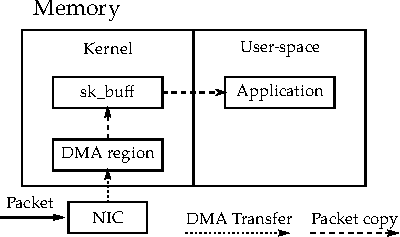
\includegraphics{figures/NAPI}
        \caption{Without PACKET\_MMAP feature}
        \label{fig:NAPI_no_MMAP}
    \end{subfigure}%
    \begin{subfigure}[t]{0.5\textwidth}
        
\includegraphics{figures/NAPI_MMAP}
        \caption{With PACKET\_MMAP feature}
        \label{fig:NAPI_MMAP}
    \end{subfigure}
    \caption{Packet transition through memory in Linux NAPI.}
    \label{fig:NAPI}
\end{figure}

The Linux network stack (with \emph{sk\_buff}) cannot be used for packet capture, because the stack takes care of all layers of the packets and delivers only the application content to the application. However, there is an option to use raw packets where the application receives and sends complete packets with all headers, including the Ethernet. The reception of raw packets uses different structure than the \emph{sk\_buff}, however, two copy operations are needed for each packet as well. Apart to the excessive copying of the packets, there is another significant performance hit. The standard API for working with packets requires to perform a system call for reception of each packet (two call when a timestamp is needed as well). Moreover, it is not possible to utilize the RSS feature provided by some NICs and process packets independently on multiple cores.

To provide an efficient way to perform packet capture using standard Linux kernel and drivers, \emph{PACKET\_MMAP}~\cite{LinuxKernelOrganization-2017-PACKETMMAP} feature was added to the kernel. It utilizes a shared buffer between the kernel and the user-space which alleviates the need to copy the packet for the second time, as show in Figure~\ref{fig:NAPI_MMAP}. Moreover, the number of packets that can be read in a single batch is not limited, which significantly lowers the number of necessary system calls and thus improves performance. Another advantage of the \emph{PACKET\_MMAP} feature is that the processing of packets can be performed by multiple threads. The distribution of packets can be performed using hash, round robin, random selection, and several other policies.

Although the Linux NAPI has evolved to support fast packet handling, there are several important performance limitations left:
\begin{itemize}
  \item The packets are copied from DMA memory region to the user-space accessible buffers.
  \item There is no support for RSS (Receive Side Scaling).
  \item There is no support for NUMA architecture awareness.
\end{itemize}

There are several frameworks that aim to remove these limitations to achieve the highest possible throughput for packet I/O operations.

\subsection{High-Speed Packet I/O Frameworks}

% lots of drivers that try to limit copying and bypass the kernel (UIO drivers)


% use related work from \section{High-Density Flow Monitoring}
% flow monitoring utilizes sequential read: dpdk vs sze2 (find paper?)
% multiqueue: supported protocols in HFE (RSS)
% timestamps
\itodo{TODO: Give a background about high-speed packet capture, lucaderi, etc.}
\itodo{find something on interrupts vs polling}
\itodo{
- Packet capture - from line to software \\
- - Technologies: PF\_RING, PF\_RING ZC, Linux NAPI, FPGA (DPDK, PF\_RING, DNA/Libzero)\\
- - http://tma.ifip.org/wordpress/wp-content/uploads/2017/06/tma2017\_paper65.pdf\\
- - http://www.beba-project.eu/public\_deliverables/BEBA\_D3.3.pdf\\
- - Timestamping: More information about packet capture can be found for example in the work of \citeauthor{Garcia-Dorado-2013-High}~\cite{Garcia-Dorado-2013-High}.\\
}

% netmap 2012
% PFQ 2012
% DPDK 2012
% PF_RING 2005
% PF_RING ZC
% SNF
% NAPATECH
% SZE2
% NAPI kernel 2.4.20 (2002), predtim byl interrupt per packet, tohle umi polling pro high load, TX_RING - raw packet access, mapped mememory also called PACKET_MMAP



% latency - not a big issue for flow monitoring, unless high precision timestamps are used


\section{Hardware Acceleration in Flow Monitoring}\label{sec:performance-hw-acceleration}

\itodo{Survey of flow caches in hardware, unsuitable for application monitoring}
% mostly for basic flow monitoring, but for the SDM

We have shown that there are many different challenges when building application flow monitoring system. Most of the described processes are performance sensitive, especially packet reception, packet parsing, and flow aggregation. To achieve application flow monitoring throughput of tens of gigabits per second, several optimization and acceleration techniques can be applied. This section focuses on these techniques. Note that we avoid the use of sampling since it degrades the quality of exported data, as shown by the authors of~\cite{Brauckhoff-2006-Impact}. Although we describe acceleration techniques, their design, and main ideas, we will not go into details about their evaluation and testing, which is out of the scope of this article. 

It has been shown by the authors of~\cite{Velan-2015-High} that standard flow monitoring can achieve more than 100 Gb/s throughput on a commodity CPU when hardware accelerated NICs are used. The work of \citeauthor{Kekely-2016-Software}~\cite{Kekely-2016-Software} shows that it is possible to utilize these NICs to achieve 100 Gb/s throughput even for application flow monitoring. We discuss both hardware accelerated techniques and software optimizations in this section. Table~\ref{tab:flow-acc-techniques} gives an overview of the discussed techniques.

% TODO abolish or update the table, it needs to point to the next section as well. It should probably contain only approaches for this section, maybe show as usable for basic/application flow monitoring
% TODO similar table in the next section
\begin{table}[ht!]
    \centering
    \begin{tabular}{|l|l|}
    \hline
    \textbf{Hardware acceleration} & \textbf{Software acceleration} \\ \hline
    Multiple reception buffers & Multithreading \\
    Packet trimming & NUMA awareness \\
    Packet header preprocessing & Flow state in parsers \\
    Flow processing offloading & Flow cache design \\
    Application identification & Flow cache timeouts \\ \hline
    \end{tabular}
    \caption{Flow Acceleration Techniques}
    \label{tab:flow-acc-techniques}
\end{table}


A field-programmable gate array (FPGA) is usually used in hardware accelerated network interface cards. It allows to parse packet headers and perform other tasks such as packet trimming or computing hashes to identify flows in the NICs. It usually supports transferring data to multiple buffers in RAM so that the software can efficiently use a multi-threading model. There are several manufacturers that provide such NICs, such as Napatech, Myricom, Mellanox Technologies, or Netcope Technologies. NICs can support hardware acceleration even without an FPGA chip, however, the capabilities are usually more limited and cannot be extended after the card is produced. For example, Intel produces many NICs without an FPGA chip that provide basic hardware acceleration such as packet hashing and transport to multiple RAM buffers.

By transferring data to multiple buffers in RAM, the NIC allows multiple CPU cores to process the data without any kind of locking mechanism. The data parsing is usually the most CPU intensive part of the application flow creation process, therefore it is very desirable to parallelize the computation. It is often necessary for the application packet parsing process to see multiple packets from the same flow. Therefore, it is desirable to store packets belonging to single flow to a single buffer in RAM, so that they are not processed by multiple different threads. To achieve this, the NIC must be able to correctly categorize packets belonging to the same flow. However, it is not necessary for the NIC to differentiate between every flow record. For example, when eight buffers are used, each flow must be sent to exactly one of the buffers. The easiest way to achieve this is to compute a three-bit hash from some of the flow-defining fields in the packet headers. IP addresses and transport layer ports are often used for this purpose, however, most manufacturers do not realize that this works incorrectly for fragmented packets. Therefore, it is better, in most scenarios, to use only IP addresses to distribute the flows to different buffers. The performance improvement achieved when using multiple buffers is directly related to the number of buffers. However, too many buffers introduce a high load on a memory controller causing the performance to be degraded. It is best to experiment with different numbers of buffers to find an optimal value for the target system. We have achieved the best results with 8-16 buffers, depending on the specific scenario and the number of CPU cores.

Memory throughput can easily become a bottleneck when data from 100\,Gb/s link are sent to RAM. One of the options to reduce the amount of processed data is to trim the received packets. Flow measurement without application protocols requires only packet headers up to the transport layer. Capturing the first 100 bytes of each packet is usually enough to contain various MPLS, VLAN, Ethernet, IPv6, and TCP headers. The rest of the packet can be discarded. The performance improvement achieved by this method depends on the average length of processed packets. However, application flow measurement requires also the packet payload. The amount of data that can be discarded varies depending on the measured application protocols. Unless the NIC has additional knowledge about measured traffic, it should not trim the packets at all for application flow measurement.

More radical way to save memory bandwidth and CPU cycles is to let the NIC extract the information required for flow monitoring and send only a special message with this information to the RAM. This process requires very specialized FPGA-based cards, such as COMBO series from CESNET. The performance gain can be quite high, as shown in~\cite{Velan-2015-High}. However, this method is not applicable for application flow measurement since application layer parsing is too complex and dynamic to be fully handled in the FPGA.

Packet trimming and packet parsing in the NIC are not usable for application flow monitoring. The main reason is that application layer parsing needs to be done in software. However, most packets do not carry application protocol headers. These packets can be processed by NIC and only extracted information transferred to software. Such a solution is proposed in~\cite{Kekely-2016-Software} and is called Software Defined Monitoring (SDM). It is based on offloading of heavy flows to the NIC. The important information from application layer is usually transferred in first N packets, where N can be expected to be lower than 20 in most cases. Therefore, after the software processing encounters the Nth packet, it instructs the NIC to process the rest of the flow. Only aggregated information about the flow is sent from NIC to software. The flow cache in the NIC is rather limited in comparison to the amount of RAM available in the software. However, only heavy flows need to be kept in this cache and it can be expired more often to reduce memory requirements. The authors show that 85 percent of traffic is observed in five percent of heavy flows. Therefore, the benefit of SDM has been shown to be an aggregation of 85 percent of packets to flow records in the NIC. This significant acceleration allows application flows to be monitored on 100\,Gb/s traffic. However, there is a downside to the SDM as well. Once a flow is offloaded to NIC, software parsers cannot observe further payloads containing subsequent application headers. For example, in the case of HTTP protocol the HTTP pipelining cannot be detected and information about further requests and responses in the same connection is lost.

Since only a small portion of all packets carry important application protocol information, it is beneficial to recognize such packets in the NIC and mark them for further processing in software. As the NIC cannot do complex application header processing, only a simple mechanism, such as pattern matching, can be utilized for packet classification. The work of the WAND Research Group~\cite{Alcock-2012-libprotoident} shows that it is possible to achieve reasonable traffic classification accuracy using only the beginning of a packet payload. Once the packets carrying application protocol headers are marked, the software parsers can process only these important packets. Moreover, other packets can be trimmed or parsed in the NIC and only important information can be passed for processing in the software. Packet classification can also benefit the SDM. When a flow is offloaded to NIC and a packet with application protocol header is matched, the processing of such a flow can be returned to the software. This approach would efficiently solve the abovementioned problem of HTTP pipelining. The accuracy and usability of pattern matching for packet classification depend on target application protocols and resource limitation of the NIC as well. Further research is needed to determine whether this method can be used for real world application flow monitoring.

\section{Flow Exporter Software Optimization}\label{sec:performance-sw-optimization}
\itodo{do not forget biflow}
\itodo{Flow expiration process - describe how flowmonexp does it and theoretical reasoning why it works quite well. Include some math to explain the ratios}
\itodo{Single packet flows can be handled separately, described by Rick and other papers}
\itodo{Flow termination per application - application specific timeouts~\cite{Rodriguez-2013-Empirical}}
\itodo{Opt-out flow processing - plugins can say whether they want to see a specific flow anymore}

The performance of flow monitoring can be greatly enhanced by offloading as much of the necessary packet processing as possible to the NIC. However, to build a high-performance flow monitoring solution the software processing must be carefully tuned as well. Moreover, the FPGA-based NICs are much more expensive than commodity NICs and cannot always be deployed. This section focuses on flow monitoring optimizations that can be achieved by careful software design and system configuration.

The development of modern CPUs has a tendency to substitute raw power (frequency) by a higher number of CPU cores. To fully utilize the potential of a multi-core CPUs and achieve high flow monitoring performance, it is necessary to create multithreaded flow monitoring software. For NICs that support storing data in multiple buffers in RAM, the solution is to have different threads process the packets from different buffers. The resulting flow records are aggregated either in a single flow cache or in multiple flow caches, one per each thread, as shown in Figure~\ref{fig:exporter-thread-schema}. In either case, it must be ensured that there is a single thread used for exporting the resulting flow records where the data from multiple processing threads are merged. The latter approach is more effective as it clearly prevents the flow cache to become a point of contention. However, when there are multiple flow caches, it is necessary to ensure that each flow is aggregated in a single flow cache. This is ensured by having the NIC correctly distribute the packets to the buffers according to their association with their respective flow. Special care needs to be taken when the application protocol parsers need to process reverse flows as well. Both directions of the communication must be processed by the same thread. Using this approach, $N+2$ threads in case the first case or $2N+1$ threads in the second case can be utilized, where $N$ is the number of buffers and the last thread is used for flow export. 

\begin{figure}[t!]
  \begin{center}
    
\includegraphics[width=\textwidth]{figures/exporter-thread-schema}
  \end{center}
  \caption{Multithreaded flow measurement with separate flow cache: a) single flow cache; b) multiple flow caches.}
  \label{fig:exporter-thread-schema}
\end{figure}

Separating packet parsing from flow cache management increases performance, however, processing application protocols may require a state of the connection to be kept. In such a case the flow cache record must be made available to the packet processing thread, which results in a use of synchronization primitives and overall performance decrease. One possible solution to this problem is to keep a different, smaller cache for chosen flow records directly in the packet processing thread. The only communication between the packet processing thread and the flow cache thread is a one-way passing of flow records, which can be done very effectively.

When a server with multiple CPUs is used, it is necessary to take care to assign each thread to correct CPU core. When the data is uploaded to RAM physically connected to different CPU than the packet processing core is running on, there is a performance hit for accessing the local memory of that CPU.

It is not effective to try every available application header parser on every packet to see which one is able to process it. When a packet from a flow was already matched by some application parser, it will usually not be matched by others. Therefore, by keeping the information about which flow is to be processed by each parser, most of the unnecessary and possibly expensive calls to application parsers can be eliminated. Moreover, when the flow is yet unmatched by any application parser, it is best to execute the application protocol parsers from the most common to the least common protocol.

One of the most performance critical parts of any flow measurement software is a flow cache. The cache needs to be designed to hold hundreds of thousands of flow records, do fast inserts, updates, and manage record expiration after active and inactive timeouts. It also needs to be robust and resilient enough to handle excessive workloads during DDoS attacks~\cite{Sadre-2012-Effects}. The flow cache design has been studied in the literature, for example in\cite{Wang-2011-Memory, Nassopulos-2014-Flow}. Although authors propose to use various data structures such as linked lists, trees, or multidimensional hashing table, our experience shows that the simplest solution is the best. The flow cache has to maintain data locality to make good use of CPU caches, therefore the dynamic structures do not perform as well as a simple hash table.

Flow cache inactive timeout expiration has a large impact on the performance, as shown in~\cite{Rodriguez-2013-Empirical, Molina-2006-Design}. The flow cache needs to be checked periodically to find and expire inactive records. However, doing the periodic checking in a separate thread requires extensive flow cache locking, which hinders the performance. Therefore, it is more efficient to dedicate part of the processing time of the flow cache thread itself to search for the inactive records. Carefully balancing the flow cache management tasks is a complex problem which offers a considerable potential for further research.

There are many other optimizations that can be performed to increase application flow monitoring performance, such as efficient flow key computation, processing packets in batches, ensuring CPU cache line alignment of flow records and so on. However, they are mostly a code micro-optimization no different from fine-tuning any other high-performance application and are out of the scope of this article.

%TODO split the anove text into the following subsections, or just have it all together
\subsection{Basic Flow Monitoring}

\subsection{Application Flow Monitoring}
\itodo{Speedup by omitting SSL/TLS processing for most application plugins}
\itodo{SW optimization: copy whole packet and parse during flow export in a separate thread - HTTP}




\section{High-Density Flow Monitoring}\label{sec:performance-high-density}
\itodo{TODO: Put in paper from IM2015}
\itodo{Say which throughput measurement method is used (sec 1)}
\itodo{What happens when processing is too slow? Which packets are dropped?}
\itodo{Measurement interference on 10x10G, need to drop on DMA, not input}

\section{Summary}\label{sec:performance-summary}